We implement the procedures in Section~\ref{sec:static} and develop a tool TaskDroid.
%the architecture of which is depicted in  Figure~\ref{fig:tool}. %where the edges represent the data flow between (sub)modules.
%\begin{figure}%[htbp]
%	\centering
%	\vspace*{-6mm}
%	\includegraphics[width = 0.9\textwidth]{tool.png}
%	\caption{Architecture of TaskDroid}\label{fig:tool}
% \vspace*{-6mm}
%\end{figure}

As depicted in Fig~\ref{fig:taskdroid}, TaskDroid comprises two modules, {\sf AMASSExtractor} and {\sf AMASSAnalyzer}.  The former module is based on ICCBot$_{AMASS}$ to build AMASS models from Android apps. The inputs of {\sf AMASSExtractor} are Android PacKage (apk)  files.
{\sf AMASSAnalyzer}  carries out the static analysis on AMASS models. {\sf AMASSAnalyzer} includes two submodules for \emph{Reachability Analyzer} and \emph{Boundedness Analyzer} 
respectively which implement the procedures given in Section~\ref{sec:static}.  Note that the Reachability submodule  %implements the procedure given in Section~\ref{sec-conf-reach}. In addition, it 
can generate witness paths for reachability.  
The Boundedness submodule %solves the stack boundedness problem. Moreover, it 
%implements the procedure given in Section~\ref{sec-boundedness}, and, 
utilises the Reachability module to generate a path starting from the main activity when the AMASS is found to be task unbounded and fragment stack unbounded.

\begin{figure}[h]
\centering
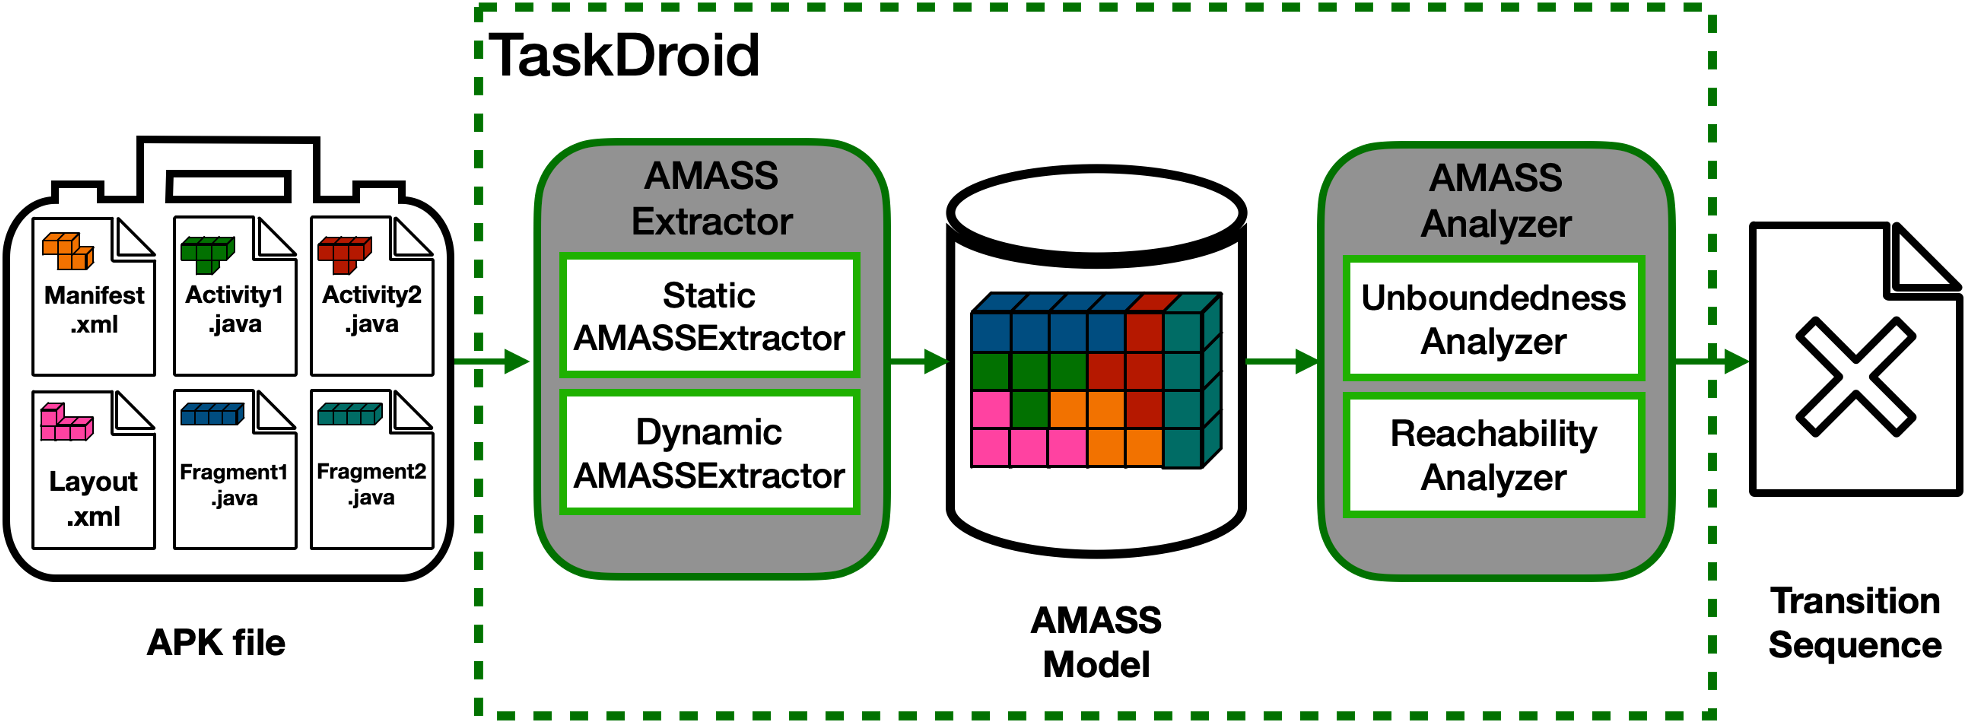
\includegraphics[scale=0.25]{taskdroid.png}
\caption{Overview of TaskDroid}
\label{fig:taskdroid}
\end{figure}
